After running the benchmark functions mentioned in Chapter \ref{chap:benchmarkSetup}, the \textit{ESP32} will serve a wireless network, on which the user can log into. While entering the default IP address (\textit{192.168.4.1}) of the \textit{ESP32}, the \textit{backend} will serve all web files. 

\begin{figure}[htbp]
	\centerline{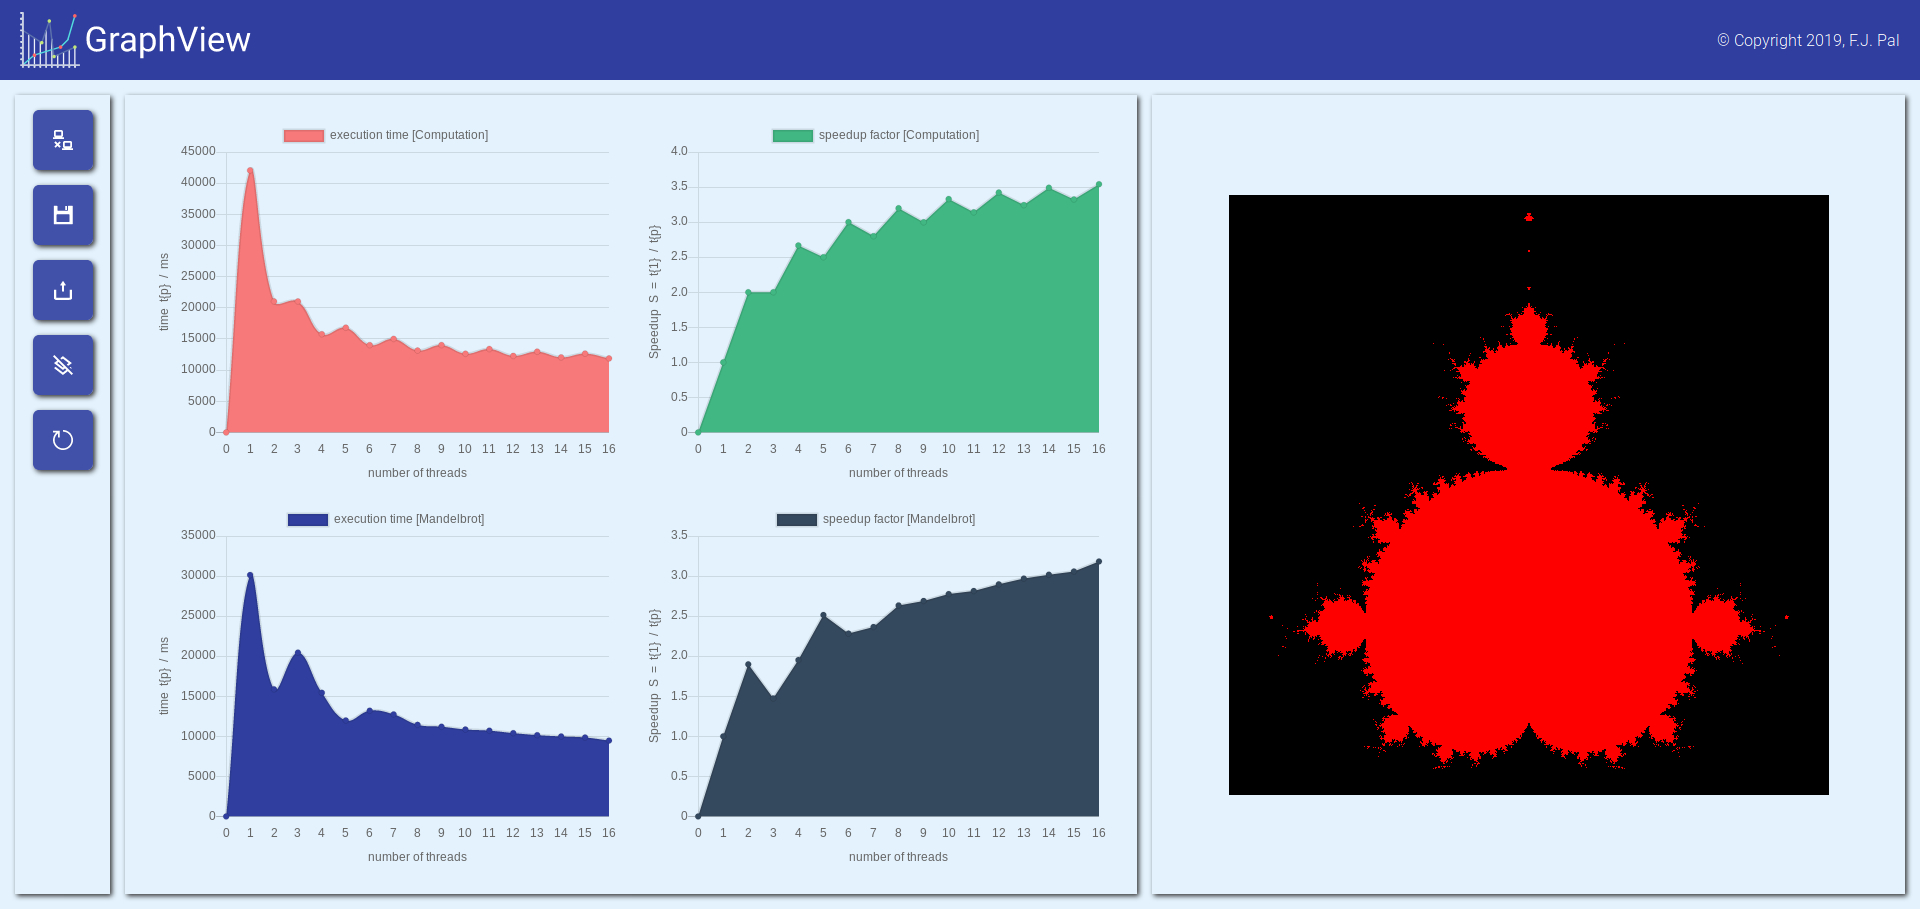
\includegraphics[width=0.95\linewidth]{images/demo.jpg}}
	\caption{ Successfully loaded \textit{frontend} with all results. }
	\label{fig:frontendResults}
\end{figure}  

The calculated results can now be loaded to the \textit{frontend} using the buttons on the left. Therefore it is necessary to open the websocket connection to the \textit{ESP32} (first button). After that we can proceed with downloading the results to our local drive by using the save button.

For both examples the chart results are quite impressive. Even after we left real time parallelism (limited to the real number of cores on the hardware system), in our case two threads running independently on different cores, it was possible to achieve a speedup. By using 62 threads for both examples, we were able to reach a maximum number of speed up of 3.65 (\textit{Mandelbrot}) and 3.7 (\textit{Computation}). Due to the fact that we run the \textit{Benchmark} on a real time operating system (\textit{FreeRTOS}), several runs of the same setup will result into almost the same results regarding execution time, because the execution time of each instruction is predictable.

The charts mentioned on the next page leads us to the assumption, that for our setup we will reach some kind of limit in speedup. But its not really comparable to the limit Amdahl's Law predicted, because we are not using real processor cores, we are dealing with thread level parallelism.

\newpage

\begin{figure}[htbp]
	\centerline{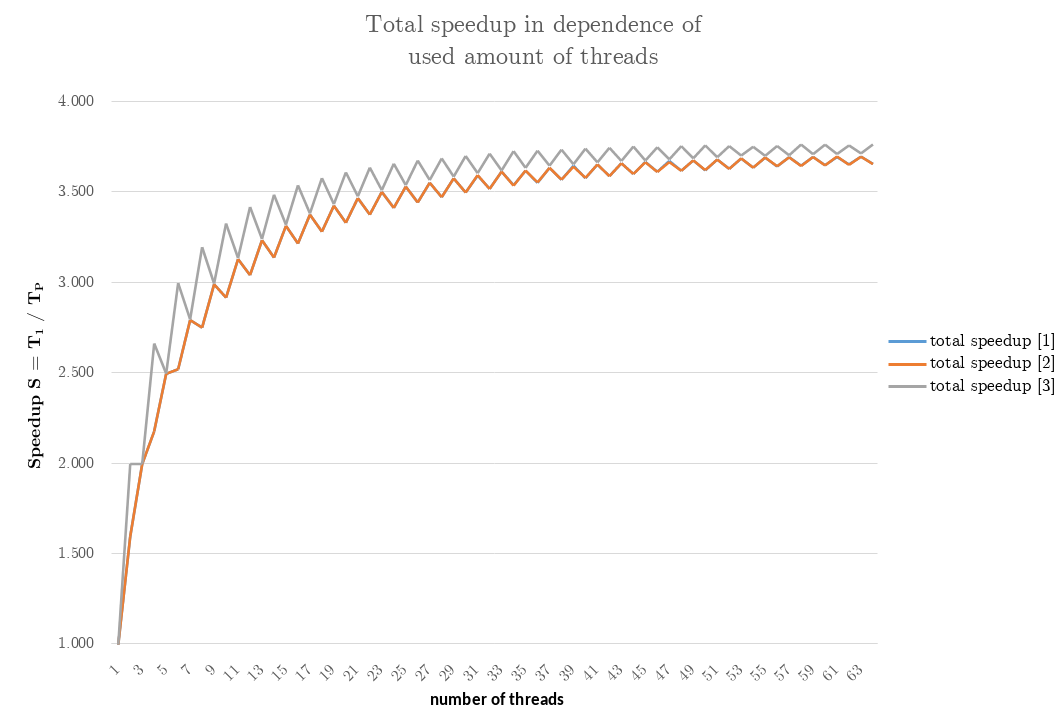
\includegraphics[width=0.8\linewidth]{images/evaluation-computation.png}}
	\caption{ Speedup factor gain for the \textit{Computation} example. }
	\label{fig:resultsComputation}
\end{figure}  

\begin{figure}[htbp]
	\centerline{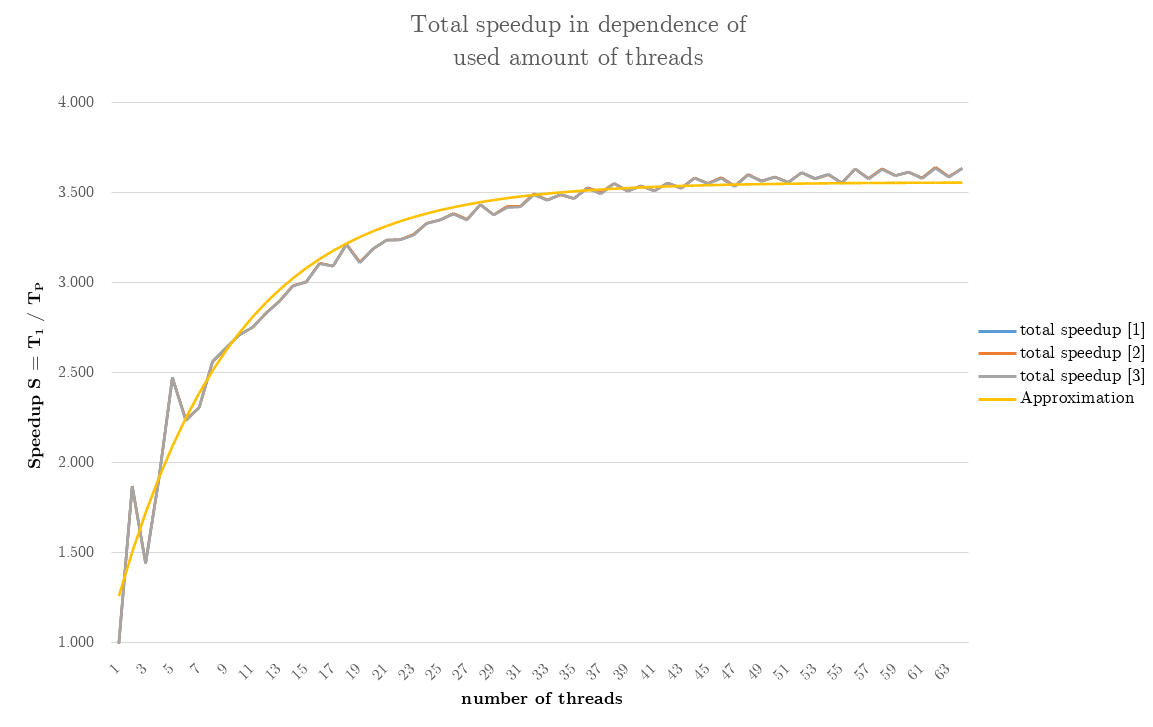
\includegraphics[width=0.8\linewidth]{images/evaluation-mandelbrot.png}}
	\caption{ Speedup factor gain for the \textit{Mandelbrot} example. }
	\label{fig:resultsMandelbrot}
\end{figure}  